\subsection{Object Document Mapper (ODM) Diagram}
\label{subsec:odm_subsec}
Because the system's database is non-relational, an Object Document Mapper (ODM) 
diagram rather than an Entity Relationship Diagram (ERD) is shown in this section.
\hfill \\

The ODM diagram is shown in Figure \ref{fig:odm}:
\begin{figure}[ht]
    \centering
    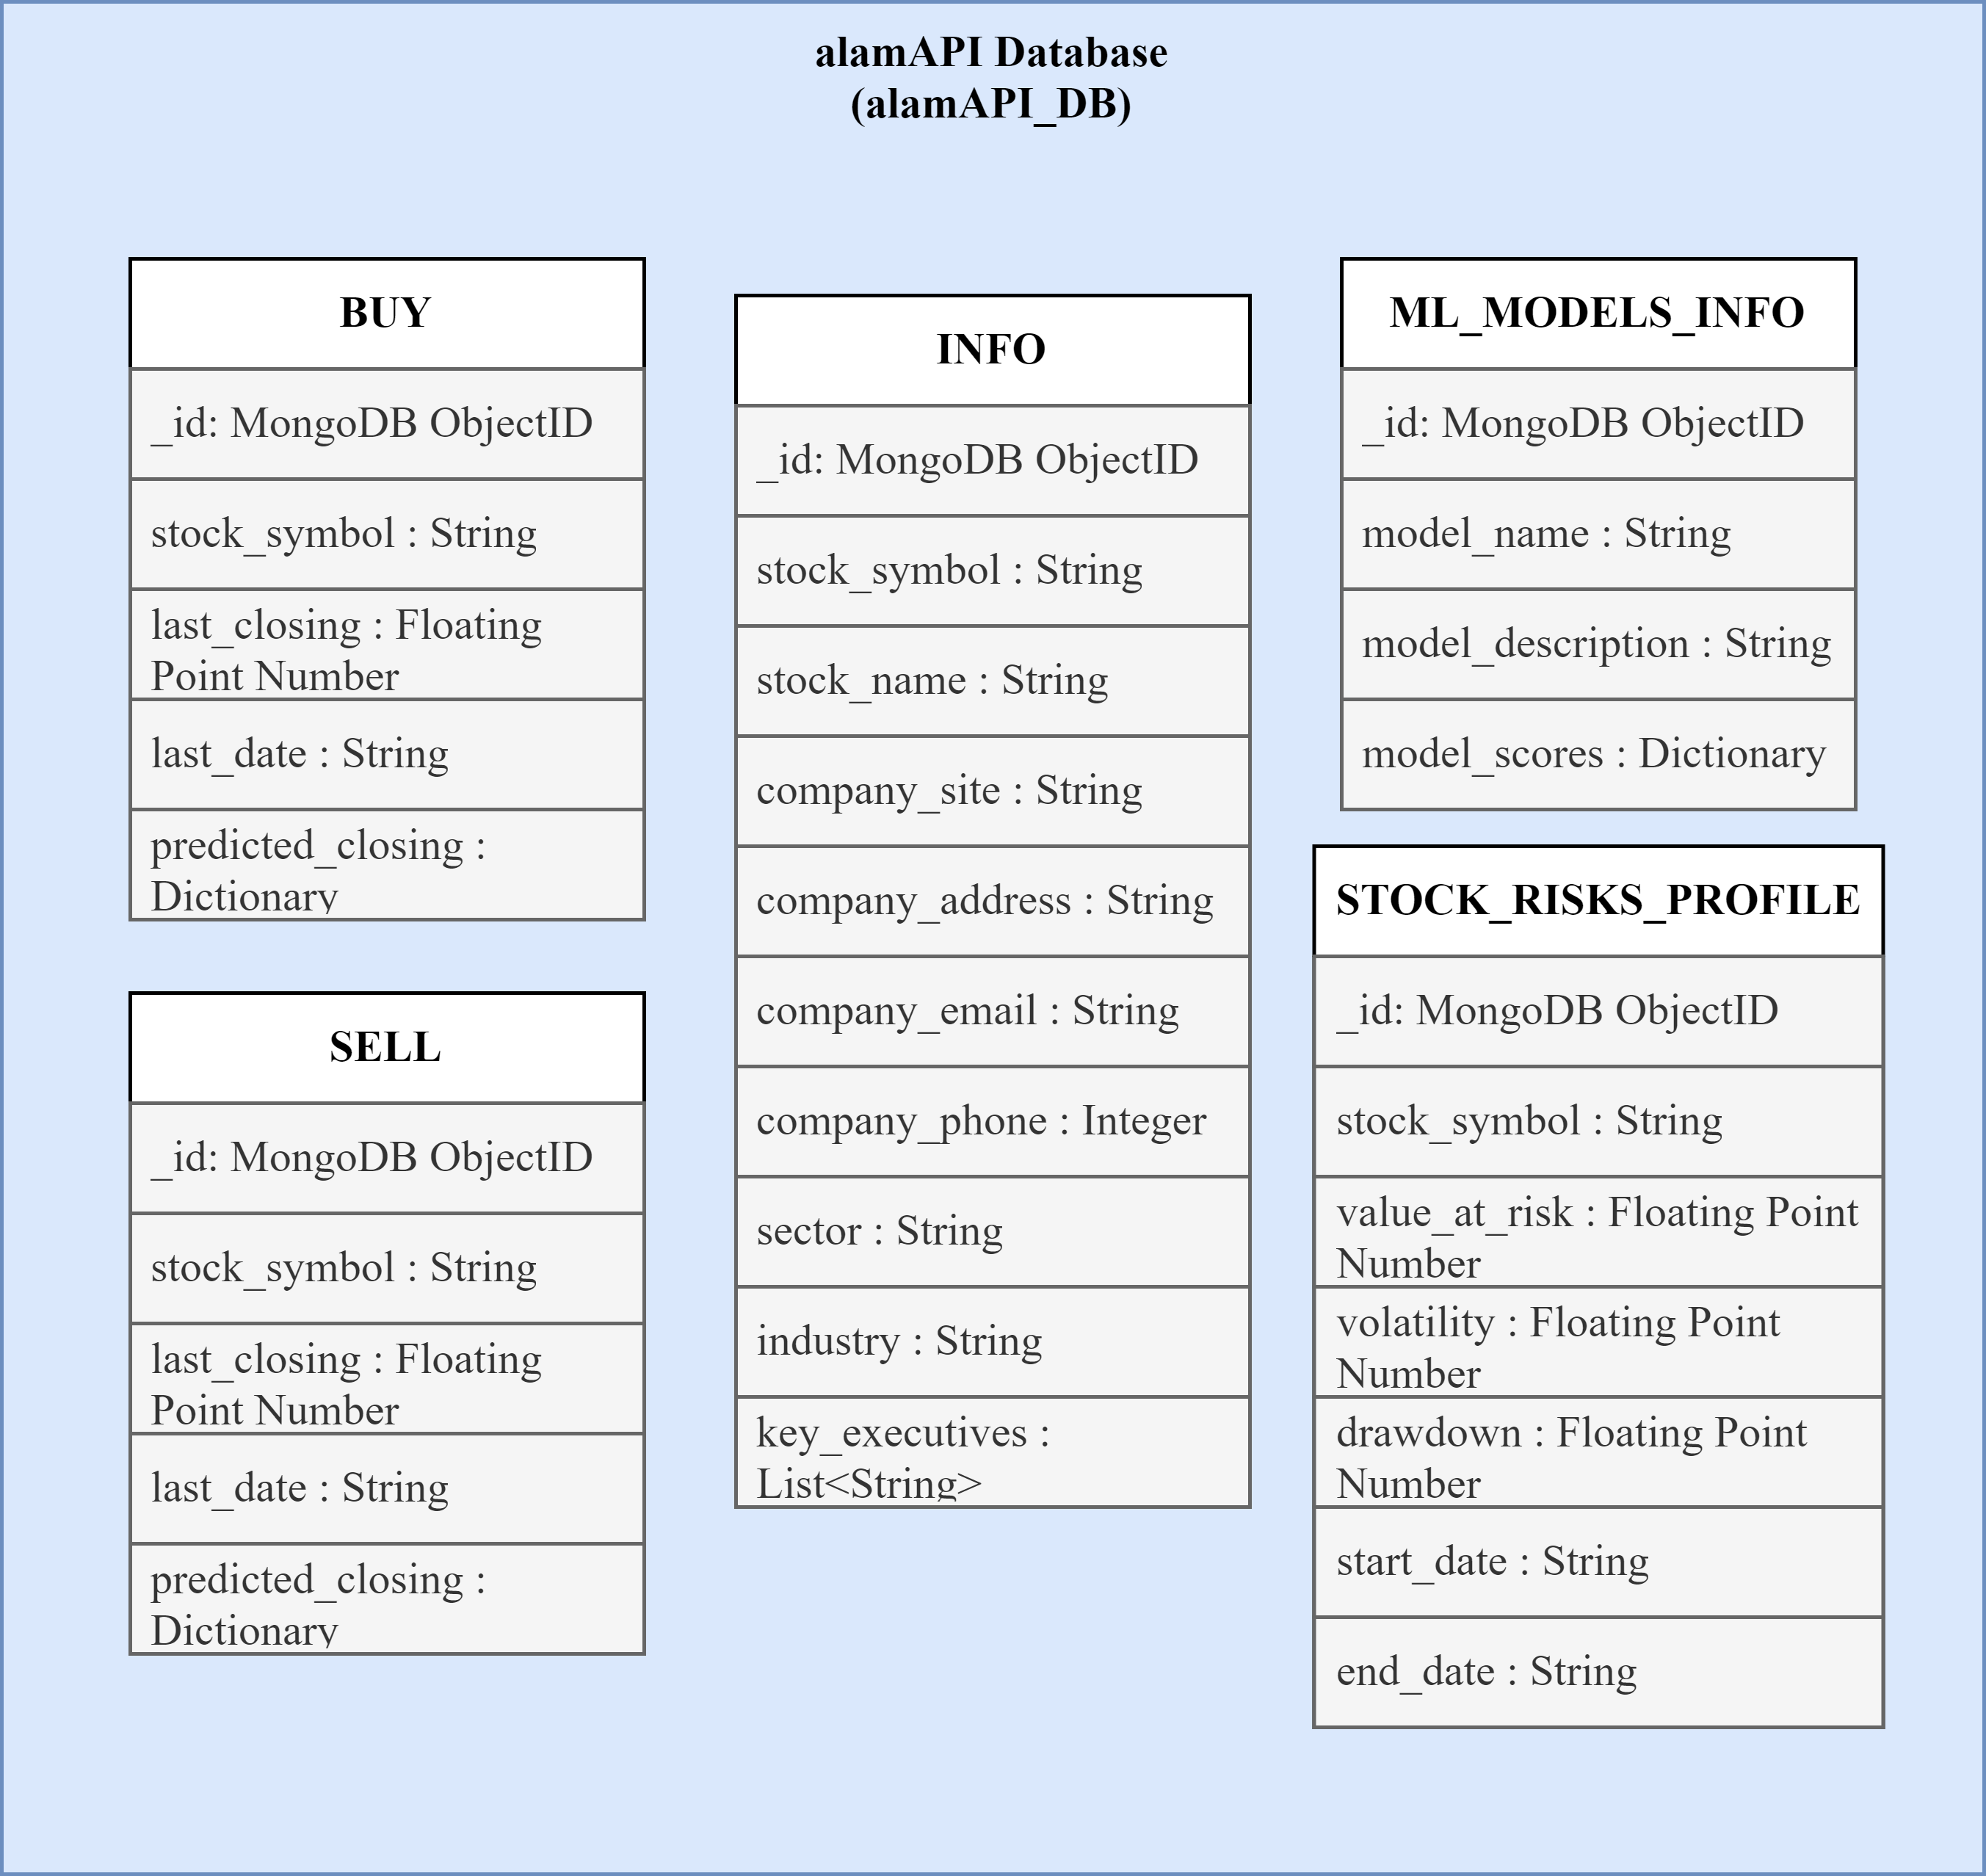
\includegraphics[width=1\textwidth]{./assets/Chapter_3/ODM/ODM.png}
    \caption{Object Document Mapper for the alamSYS Database}
    \label{fig:odm}
\end{figure}
\FloatBarrier
As shown from the Figure \ref{fig:odm}, the "alamAPI\_DB" is the database
name of the system. Where it is composed of five collections namely:
\begin{itemize}
    \item[(a)] Buy – this collection contains all the stocks that the 
    data processor predicted and classified as a stock to buy. A sample
    of which is presented in Figure \ref{fig:odm_buy_sample}.
    \begin{figure}[ht]
        \centering
        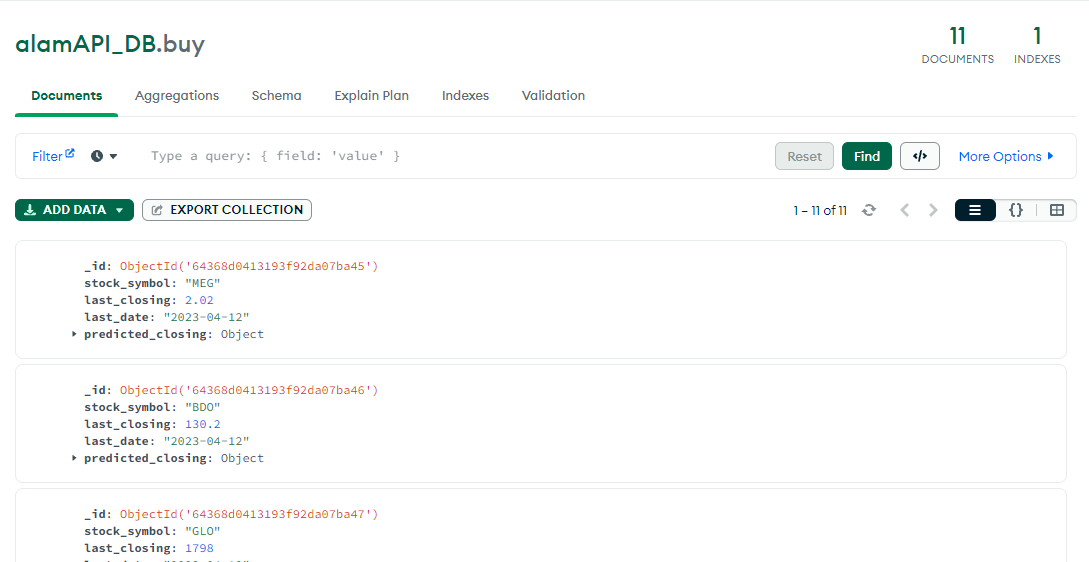
\includegraphics[width=1\textwidth]{./assets/Chapter_3/ODM/ODM_Buy_Sample.png}
        \caption{Sample Buy Collection from the alamSYS Database}
        \label{fig:odm_buy_sample}
    \end{figure}
    \FloatBarrier

    \item[(b)] Sell – this collection contains all the stocks that the
    data processor predicted and classified as a stock to sell. a
    sample of which is presented in Figure \ref{fig:odm_sell_sample}.
    \begin{figure}[ht]
        \centering
        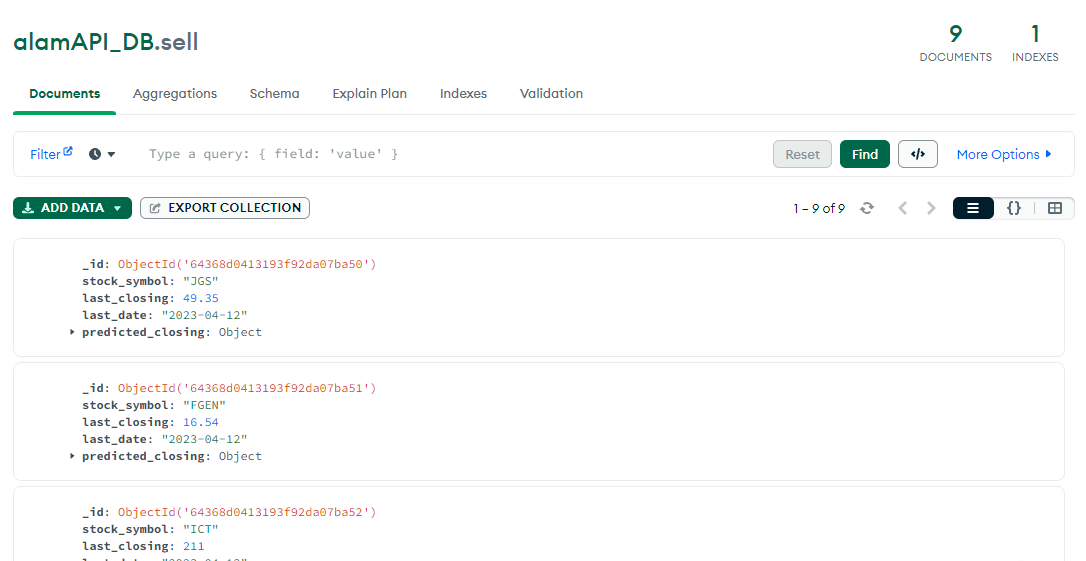
\includegraphics[width=1\textwidth]{./assets/Chapter_3/ODM/ODM_Sell_Sample.png}
        \caption{Sample Sell Collection from the alamSYS Database}
        \label{fig:odm_sell_sample}
    \end{figure}
    \FloatBarrier

    \item[(c)] Info – this collection contains the general and relevant 
    information about a stock, or the general company information. Such as
    the stock symbol, stock name, company site, company address, company email,
    company phone number, sector, industry, and the company's key executives. Where
    all of this information are gathered from their official listing accessed in the
    database of the Philippine Stock Exchange (PSE). A sample of which is presented
    in Figure \ref{fig:odm_info_sample}.
    \begin{figure}[ht]
        \centering
        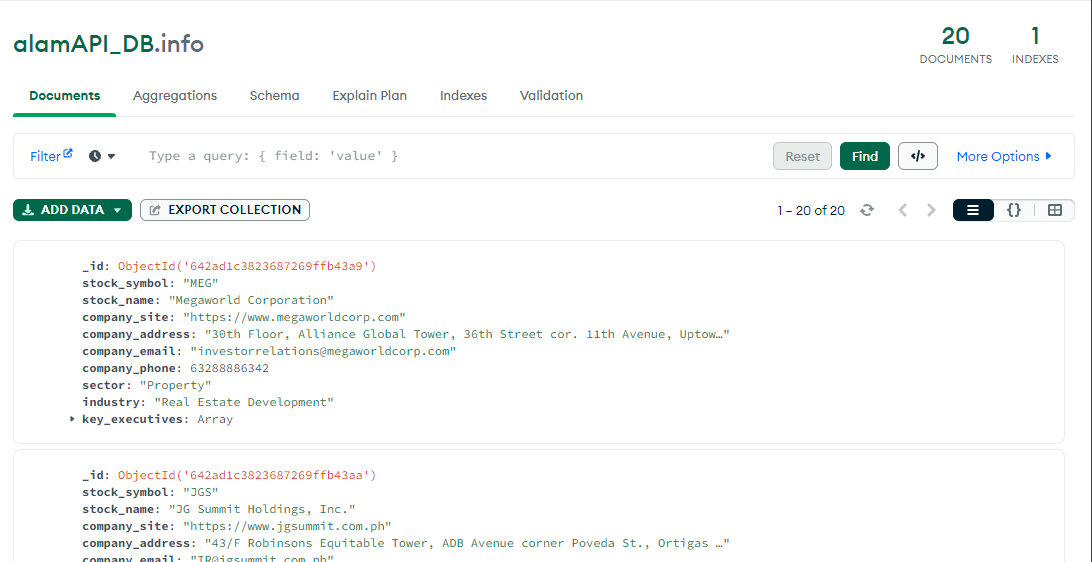
\includegraphics[width=1\textwidth]{./assets/Chapter_3/ODM/ODM_Info_Sample.png}
        \caption{Sample Info Collection from the alamSYS Database}
        \label{fig:odm_info_sample}
    \end{figure}
    \FloatBarrier

    \item[(d)] Machine Learning (ML) Models Info – this collection contains
    the details about the Machine Learning Model/s deployed in the system. For the current
    alamSYS, only one model is deployed, which is the DMD-LSTM model. A sample of which
    is presented in Figure \ref{fig:odm_ml_sample}.
    \begin{figure}[ht]
        \centering
        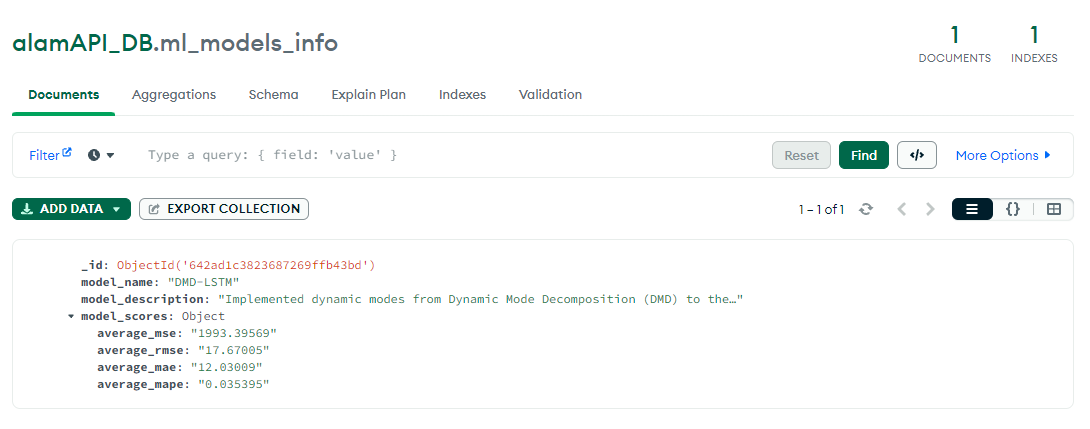
\includegraphics[width=1\textwidth]{./assets/Chapter_3/ODM/ODM_ML_Sample.png}
        \caption{Sample ML Models Info Collection from the alamSYS Database}
        \label{fig:odm_ml_sample}
    \end{figure}
    \FloatBarrier

    \item[(e)] Stock Risks Profile  - this collection contains the details about the risk profiles
    for each stock. A sample of which is presented in Figure \ref{fig:odm_ml_sample}.
    \begin{figure}[ht]
        \centering
        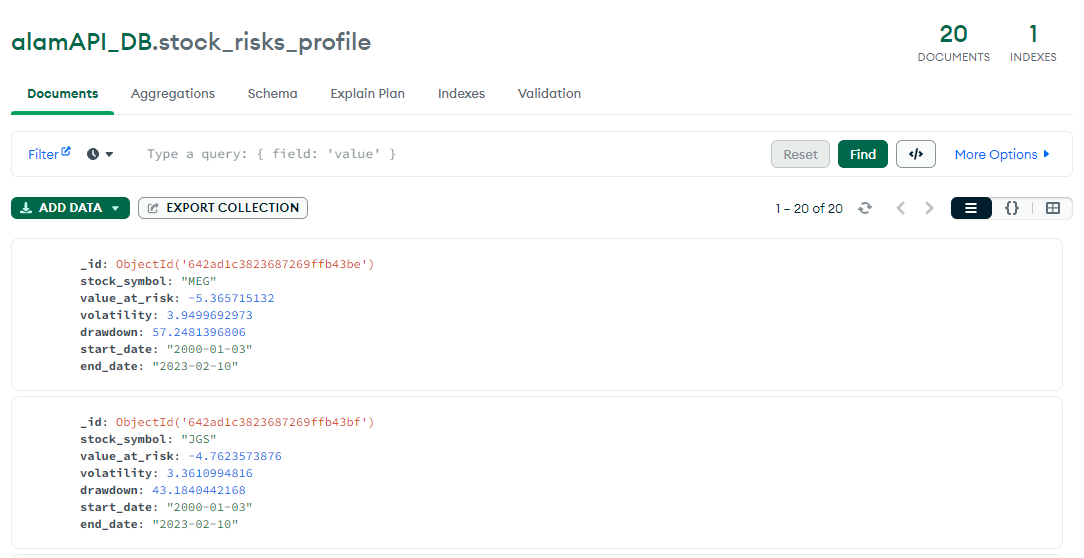
\includegraphics[width=1\textwidth]{./assets/Chapter_3/ODM/ODM_Risks_Sample.png}
        \caption{Sample Stock Risks Profile Collection from the alamSYS Database}
        \label{fig:odm_ml_sample}
    \end{figure}
    \FloatBarrier

\end{itemize}
\textit{Note that each collection are their own separate entities, 
hence the database is called non-relational, as the documents are not in 
any way related to each other.}
\hfill \\